\section{Основные понятия теории графов}
Перед постановкой самой задачи раскраски графов следует вспомнить основные определения, которые можно найти, например, в \cite{Alexeev,Harary}.

\begin{definition}\label{d1}
	\textit{Обыкновенным графом} называется пара $G=\left(V,E\right),$ где $V$ --- конечное множество и $E$ --- множество неупорядоченных пар различных элементов из множества $V.$ Элементы множества $V$ называются \textit{вершинами} графа, а элементы множества $E$ --- его рёбрами. 
\end{definition}

\begin{definition}
	Если в графе $G$ имеется ребро $e = \left( x,y\right) ,$ то говорят, что вершины $x$ и $y$ смежны в этом графе. Ребро $e$ инцидентно каждой из вершин $x$ и $y,$ а каждая из этих вершин инцидентна этому ребру.
\end{definition}


\begin{figure}[H]
	\centering
		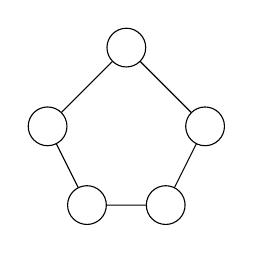
\begin{tikzpicture}
		\draw (1,0) -- (0,-1) -- (0.5,-2) -- (1.5,-2) -- (2,-1) -- (1,0);
		
		\draw[fill = white] (1,0) circle (7pt);
		\draw[fill = white] (0,-1) circle (7pt);
		\draw[fill = white] (2,-1) circle (7pt);
		\draw[fill = white] (0.5,-2) circle (7pt);
		\draw[fill = white] (1.5,-2) circle (7pt);
	\end{tikzpicture}\qquad
	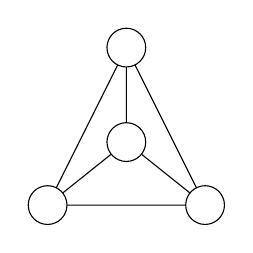
\begin{tikzpicture} 
		\draw (1,-1.2) -- (1,0) -- (0,-2) -- (2,-2) -- (1,-1.2) -- (0,-2); 
		\draw (1,0) -- (2,-2);
		\draw[fill=white] (1,0) circle (7pt); 
		\draw[fill=white] (1,-1.2) circle (7pt);
		\draw[fill=white] (0,-2) circle (7pt);
		\draw[fill=white] (2,-2) circle (7pt);
	\end{tikzpicture}\qquad
	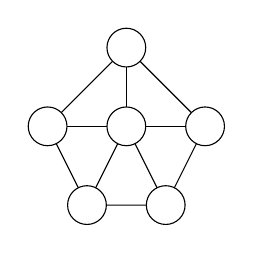
\begin{tikzpicture}
		\draw (1,0) -- (0,-1) -- (0.5,-2) -- (1.5,-2) -- (2,-1) -- (1,0);
		\draw (1,-1) -- (1,0);
		\draw (1,-1) -- (0,-1);
		\draw (1,-1) -- (2,-1);
		\draw (1,-1) -- (0.5,-2);
		\draw (1,-1) -- (1.5,-2); 
		
		\draw[fill = white] (1,0) circle (7pt);
		\draw[fill = white] (0,-1) circle (7pt);
		\draw[fill = white] (1,-1) circle (7pt);
		\draw[fill = white] (2,-1) circle (7pt);
		\draw[fill = white] (0.5,-2) circle (7pt);
		\draw[fill = white] (1.5,-2) circle (7pt);
	\end{tikzpicture}
	\caption{Пример графов $C_5,$ $W_4$ и $W_6.$}
	\label{pic5}
\end{figure}

Пример картинки:

\begin{figure}[H]
	\centering
	
\includegraphics{TimeAlg.eps}
	\caption{Время работы алгоритмов \texttt{GREEDY} и \texttt{DSATUR}}
\end{figure}